\subsection{Nghiên cứu và lựa chọn mô hình phát triển phần mềm}
Việc lựa chọn quy trình phát triển phần mềm phù hợp quyết định đến khả năng quản lý rủi ro và tiến độ của dự án. Nhóm đã nghiên cứu một số mô hình phổ biến sau:

    \subsubsection{Mô hình Thác nước (Waterfall)}
    \begin{figure}[H]
        \centering
        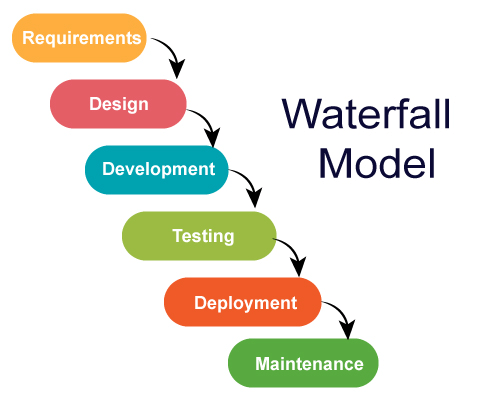
\includegraphics[width=0.7\linewidth]{3.Nghiên cứu/Images/WaterFall.png}
        \caption{Mô hình Waterfall}
        \label{fig:placeholder}
    \end{figure}

    Waterfall model được coi là mô hình phát triển phần mềm đầu tiên được sử dụng. Lý do việc mô hình này được gọi là thác nước vì các giai đoạn phát triển được thực hiện tuần tự và nối tiếp nhau, như một dòng nước chảy. Mỗi giai đoạn hoàn thành trước khi giai đoạn tiếp theo bắt đầu và không có sự quay lại. Do tính chất này, mỗi giai đoạn của mô hình thác nước phải được xác định chính xác.
    
    \subsubsection{Mô hình Agile}
    \begin{figure} [H]
        \centering
        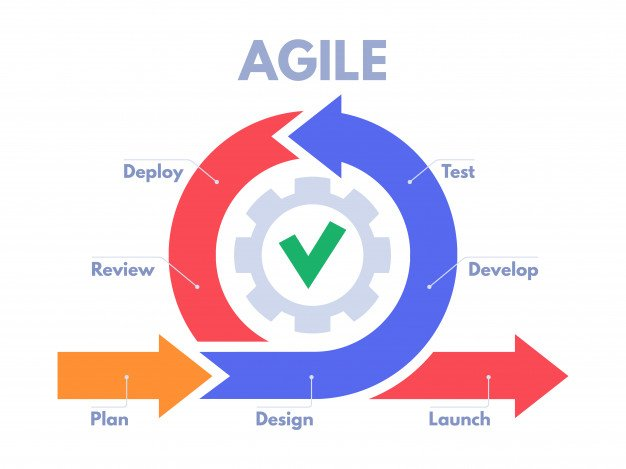
\includegraphics[width=0.7\linewidth]{3.Nghiên cứu//Images/Agile.png}
        \caption{Mô hình Agile}
        \label{fig:placeholder}
    \end{figure}
    Mô hình Agile là một phương pháp phát triển phần mềm linh hoạt. Agile model được tạo ra dựa trên 2 mô hình: Iterative (Lặp lại) và Incremental (Tăng dần). Nó tập trung vào việc phân phối sản phẩm thông qua các chu kỳ phát triển ngắn (gọi là sprint) và thường xuyên nhận phản hồi từ khách hàng. \\
    
    Agile giúp nhóm phát triển dễ dàng thích nghi với các thay đổi yêu cầu, đồng thời cải thiện chất lượng sản phẩm liên tục.
    
    \subsubsection{Quy trình Scrum}
    \begin{figure} [H]
        \centering
        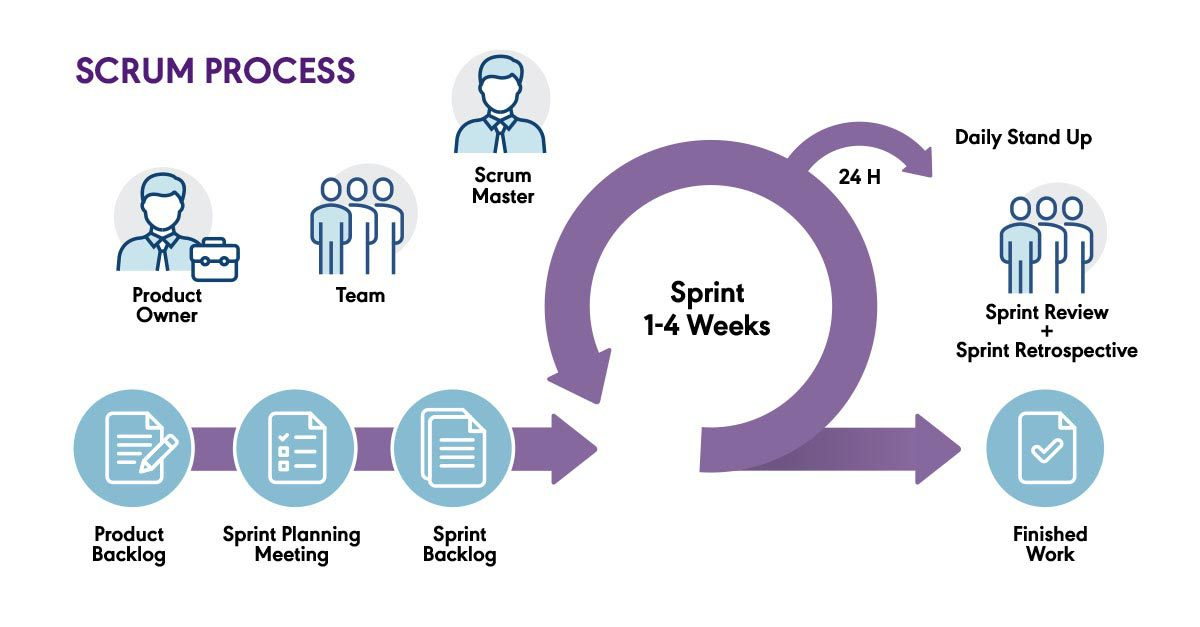
\includegraphics[width=0.75\linewidth]{3.Nghiên cứu//Images/Scrum.png}
        \caption{Scrum Process}
        \label{fig:placeholder}
    \end{figure}
    Scrum là một “khung quản lý dự án” được áp dụng rất rộng rãi từ những dự án đơn giản với một nhóm phát triển nhỏ cho đến những dự án có yêu cầu rất phức tạp với hàng trăm người tham gia. Ngoài ra, Scrum Process cũng phù hợp với những dự án đòi hỏi khung thời gian cố định. \\

    Trong Scrum, công việc sẽ được chia nhỏ thành nhiều giai đoạn gọi là Sprint. Mỗi Sprint chỉ kéo dài từ 1 đến 4 tuần, không quá một tháng. Đầu Sprint sẽ lên kế hoạch làm những yêu cầu nào rồi thực hiện code và test. Cuối Sprint là một sản phẩm hoàn thiện cả code lẫn test có thể demo và chạy được.

    \subsubsection{So sánh các mô hình phát triển dự án phần mềm}
    Mỗi mô hình phát triển dự án đều có các đặc điểm nổi trội riêng, Do đó để phân tích rõ hơn việc lựa chọn giữa các mô hình phát triển để thực hiện dự án, dưới đây là bảng so sánh điểm mạnh và điểm yếu giữa các mô hình:
    \begin{table}[H]
    \centering
    \begin{tabular}{|p{2cm}|p{6cm}|p{6cm}|}
    \hline
    \textbf{Mô hình} & \textbf{Điểm mạnh} & \textbf{Điểm yếu}\\
    \hline
    \textbf{Waterfall} & 
            $\bullet$ Phù hợp với dự án nhỏ và ngắn hạn
            
            $\bullet$ Dễ quản lý, có kế hoạch rõ ràng từ đầu.
            
            $\bullet$ Có sự ổn định cao, ít thay đổi và xác định yêu cầu rõ ràng.
        & 
            $\bullet$ Rất khó để quay lại giai đoạn nào khi nó đã kết thúc
            
            $\bullet$ Ít tính linh hoạt và phạm vi điều chỉnh của nó khá là khó khăn, tốn kém.
         \\
    \hline
    \textbf{Agile} & 
            $\bullet$ Tăng cường khả năng làm việc nhóm.
            
            $\bullet$ Các chức năng được rõ ràng và dễ quản lý.
            
            $\bullet$ Có tính linh hoạt cao.
        & 
            $\bullet$ Không phù hợp với các dự án phức tạp.
            
            $\bullet$ Phụ thuộc vào yếu tố bên ngoài
            
            $\bullet$ Khó kiểm soát tiến độ và deadline.
            
            $\bullet$ Dễ mất định hướng nếu không có kế hoạch rõ ràng.
         \\
    \hline
    \textbf{Scrum} & 
            $\bullet$ Quản lý tiến độ chặt chẽ theo Sprint.
            
            $\bullet$ Theo dõi hiệu suất làm việc rõ ràng.
            
            $\bullet$ Phân chia công việc cụ thể, rõ trách nhiệm.
        & 
            $\bullet$ Nhiều họp, tốn thời gian quy trình.
            
            $\bullet$ Không linh hoạt như Agile thuần.
            
            $\bullet$ Hạn chế việc thay đổi đột ngột giữa Sprint.
         \\
    \hline
    \end{tabular}
    \caption{Bảng So sánh các mô hình phát triển dự án phần mềm}
\end{table}
    Qua bảng phân tích trên, nhóm nhận thấy các đặc điểm của mô hình Scrum là phù hợp với dự án của nhóm nhất. Do đó nhóm quyết định sử dụng mô hình Scrum để phát triển dự án.

